\section{Experimental Evaluation}\label{sec:eval}

\subsection{Methodology and Testbed Cost}\label{sec:metrics}
We report latency, throughput, on-chain gas, revocation exposure (requests accepted after revocation), per-tier acceptance of legitimate and attacking requests, quorum behaviour, recall capacity and degraded-mode behaviour. Three limits apply throughout. (i) Testbed timings are \emph{compute-bound}: they exclude network, block time and multi-node consensus. (ii) Sections~\ref{sec:scaling}--\ref{sec:outage_eval} use \emph{synthetic} devices, signals and attacks, so they characterize policy mechanics under stated overlaps; Section~\ref{sec:real_eval} replaces the behavioural signal with detector scores from real TON\_IoT traffic, while posture and network context stay synthetic. (iii) One two-vCPU host was used.

\paragraph{Latency.}\label{sec:scaling} Mean authorization latency is 0.120--0.197\,ms and registration 0.173--0.286\,ms; beyond 200 devices latency stays flat as the fleet grows eightfold. This fits a constant per-request cost dominated by one Ed25519 verification, with 3{,}700--6{,}200 decisions/s. Thirty repeats at 400 devices give $0.133\pm0.013$\,ms for authorization (95\% CI 0.128--0.138) and $0.184\pm0.019$\,ms for registration. Over 20{,}000 sequential decisions p50 is 0.124\,ms, p95 0.188, p99 0.247 and p99.9 0.932\,ms (4.3\,ms maximum). The fast-path PEP, which verifies the device signature and the oracle attestation, takes $0.261\pm0.022$\,ms against $0.134\pm0.020$\,ms for the contract model with one signature (10 runs of 2{,}000 mixed T0/T2 requests), about 3{,}800 decisions/s on one core. This is a cost, not a gain: the fast path needs no transaction, gas or block, and what that is worth depends on network and consensus latency that this test did not measure.

\paragraph{Gas.}\label{sec:gas} Table~\ref{tab:gas} lists gas measured over 50 devices on the Hardhat EVM (deterministic, s.d.\ below 10). Registration costs about 215k gas and a full audited decision about 70k, mostly one \texttt{ecrecover} and one new nonce slot. Replay (41.8k) and revoked-device (39.6k) denials exit early. The industrial additions cost almost nothing: the anomaly-gate, strict-mode and threshold outcomes are all within 0.3\% of the base decision. Anchoring a decision-log root costs 70.8k gas the first time and 53.7k in steady state, or 54 gas per decision at 1{,}000 decisions per root, about three orders of magnitude below deciding each on-chain. A 30M-gas block holds at most 424 audited decisions (about 212 per second at a 2\,s block period) or 139 registrations; this is an upper bound, not a measured throughput (Section~\ref{sec:besu_eval}), and it is why only T2--T3 are decided on-chain. The audited decision now also checks the attestation's expiry time, which is included in these figures.

\begin{table}[t]
\centering
\caption{Measured gas per operation (Hardhat EVM, solc 0.8.24, 50 devices)}
\label{tab:gas}
\scriptsize
\begin{tabular}{@{}lrr@{}}
\toprule
\textbf{Operation} & \textbf{Mean gas} & \textbf{Std.} \\
\midrule
\texttt{registerDevice} & 214{,}973 & 8.7 \\
\texttt{suspendDevice} & 32{,}710 & 2.9 \\
\texttt{reinstateDevice} & 32{,}876 & 2.9 \\
\texttt{revokeDevice} & 58{,}799 & 2.9 \\
\texttt{evaluateAccess} (ALLOW) & 70{,}751 & 5.7 \\
\texttt{evaluateAccess} (STEP\_UP) & 70{,}793 & 6.4 \\
\texttt{evaluateAccess} (DENY, bad oracle sig.) & 70{,}521 & 7.1 \\
\texttt{evaluateAccess} (DENY, replay) & 41{,}809 & 5.7 \\
\texttt{evaluateAccess} (DENY, revoked) & 39{,}589 & 8.0 \\
\midrule
Deploy \texttt{IdentityRegistry} & 1{,}424{,}212 & -- \\
Deploy \texttt{ZeroTrustAccess} & 1{,}105{,}598 & -- \\
\texttt{definePolicy} (2 classes) & 97{,}805 & -- \\
\bottomrule
\end{tabular}
\end{table}

\subsection{Tiered Policy: Legitimate Acceptance and Attack Acceptance}\label{sec:tiers_eval}
Table~\ref{tab:tiersres} runs 4{,}000 legitimate requests (5\% with a process upset) and 4{,}000 requests of each attack population through the four tiers, with threshold alone and with the full policy (gate and strict mode). Eligibility is by device class, so legitimate denominators shrink with the tier (4{,}000, 3{,}713, 1{,}145, 858). Naive compromise is denied everywhere. At T0 a signal-spoofing attacker is accepted under any policy, by design, since T0 is read-only. Where consequences are high the gate and strict mode matter: at T2 the full-spoof attacker falls from 100\% to 0\% accepted and the stealthy attacker from 98.5\% to 60.9\%; at T3 from 52.4\% to 0\% and from 52.2\% to 13.6\%. The price is that legitimate allowance drops from 99.9\% to 97.8\% at T2 and from 96.0\% to 94.8\% at T3 (5.2\% denied outright), because upset requests exceed the gate and strict mode refuses borderline scores. In an ablation, the full score separates partial and stealthy mimicry with AUC 0.993 and 0.895, whereas dropping the behavioural signal leaves both at 0.50. Posture and network are drawn from the same ranges for both populations, so removing them raises AUC. This argues for adaptive weighting, not for real posture being uninformative.

\begin{table}[t]
\centering
\caption{Per-tier results: legitimate requests allowed and attacker requests accepted (\%), threshold alone $\to$ full policy ($\theta$ min.\ trust, $g$ anomaly gate)}
\label{tab:tiersres}
\scriptsize
\setlength{\tabcolsep}{2.2pt}
\begin{tabular}{@{}lccrrr@{}}
\toprule
\textbf{Resource} & $\theta$ & $g$ & Legit. & Stealthy & Spoof \\
\midrule
telemetry.read (T0) & 0.50 & 1.00 & 100.0$\to$100.0 & 100.0$\to$100.0 & 100.0$\to$100.0 \\
historian.write (T1) & 0.55 & 0.60 & 100.0$\to$100.0 & 100.0$\to$100.0 & 100.0$\to$74.7 \\
plc.setpoint.write (T2) & 0.70 & 0.30 & 99.9$\to$97.8 & 98.5$\to$60.9 & 100.0$\to$0.0 \\
plc.firmware.update (T3) & 0.78 & 0.20 & 96.0$\to$94.8 & 52.2$\to$13.6 & 52.4$\to$0.0 \\
\bottomrule
\end{tabular}
\end{table}

\paragraph{Gate level.}\label{sec:gate_eval} Fig.~\ref{fig:iiotres}(b) sweeps the gate. At a 5\% upset rate a gate of 0.30 blocks 40.1\% of stealthy mimicry and 100\% of full spoofing while denying 2.3\% of legitimate requests. A gate of 0.20 blocks 80.4\% of stealthy mimicry at 3.8\% denials, and 0.40 blocks none and lets 25\% of full spoofing through. At a 15\% upset rate, gates of 0.30 and 0.20 deny 7.4\% and 12.2\% of legitimate requests. The operating point depends on how noisy legitimate behaviour is, and an attacker that keeps its anomaly below the gate is accepted, as Proposition~\ref{prop:bound}(d) predicts.

\subsection{Evaluation on Real Traffic: TON\_IoT}\label{sec:real_eval}
The synthetic study fixes the anomaly distributions by hand, so we repeat the central experiments with $A$ produced by detectors on a public dataset. TON\_IoT provides labelled IIoT telemetry \cite{alsaedi2020ton} and network flows \cite{moustafa2021network}, whose heterogeneity is analysed in \cite{booij2022ton}. We used four telemetry files and the network file (211{,}043 flows, 190{,}474 after removing 20{,}569 exact duplicates; nine attack types plus normal traffic). Features exclude IP addresses, source ports and, for telemetry, dates and times (normal and attack records were collected on different days). A gradient-boosted classifier (supervised) and an Isolation Forest trained on normal records only (unsupervised) are evaluated on a stratified 70/30 split over five seeds; to approximate unseen attacks we also train the classifier with one attack type left out. The attack probability is $A\in[0,1]$. Legitimate requests carry the score of a normal test flow; attackers carry the score of an attack flow and spoof posture and network context to 1 (the full-spoof attacker of Section~\ref{sec:devsim}). Posture, network context and the reliability warm-up stay synthetic, and because the files share no device identifier, assigning a flow-derived score to a device is arbitrary. The four tiers are used unchanged.

\emph{Telemetry alone is a weak signal.} Only the Weather file separates attacks usefully (supervised AUC 0.972, Isolation Forest 0.819); Modbus gives 0.623 and 0.498, and Thermostat and Fridge are near chance. Before whitespace stripping, one Fridge column carries label-specific padding that gives a perfect AUC, an encoding artefact, so we strip all strings before training. A plant's behavioural signal should come from traffic, not only from sensor values.

\emph{Network flows are a strong signal, with a caveat.} On flows the supervised classifier reaches AUC 0.9999 and the Isolation Forest $0.916\pm0.004$ (0.813 for DDoS to 0.956 for password attacks). Read the near-perfect supervised value as an upper bound, since random splits of a benchmark whose attacks come from a few hosts are optimistic. With a type withheld, AUC against normal traffic stays at 0.990--1.000, but the share of that type scored above 0.5 falls to 65.4\% for ransomware and 73.7\% for man-in-the-middle, against 93--100\% for most others. Legitimate flows mostly score near zero (median 0.0003) but the tail is heavy (99th percentile 0.27, 99.9th 0.96).

\emph{Policy on real scores.} Table~\ref{tab:realpolicy} gives attacker requests accepted, averaged over the nine attack types and for the worst type. First, the full policy costs legitimate traffic little: allowance falls from 99.7, 99.5 and 99.0\% to 99.6, 98.8 and 98.4\% at T1, T2 and T3. Second, for seen attack types the gate matters at T1 (mean acceptance 100\% $\to$ 0.7\%, worst 4.9\%), whereas at T2 and T3 the high thresholds already reject nearly all such flows (1.1\% and 0.6\% with threshold alone). A real detector scores them near 1, and Proposition~\ref{prop:bound}(d) then gives $T\approx0.7$ or below. This corrects the synthetic study, which overstated how often the threshold alone fails on seen attacks. Third, for held-out types residual acceptance grows to 11.9\% (T1), 7.9\% (T2) and 6.6\% (T3) on average and to 41.6\%, 33.9\% and 35.8\% for the worst type (ransomware): a policy that depends on a detector inherits its blind spots. Fourth, an adaptive attacker that observes the detector and sends only its best-scoring flows is far more dangerous. The lowest-scoring 10\% of a held-out type's flows give mean acceptance of 59.4, 37.9 and 29.0\% at T1--T3, and the best 1\% give 76.5, 74.7 and 58.2\%. This assumes the attacker can query the detector and choose a score, a strong capability, so these are worst cases. A gate of 0.30 on the real scores denies 1.0\% of legitimate flows and blocks 99.9\% of seen and 94.6\% of held-out attack flows. Detector hyper-parameters were library defaults and none was tuned on these results.

\begin{table}[t]
\centering
\caption{Attacker requests accepted (\%) with real TON\_IoT anomaly scores: mean over nine attack types and worst single type; threshold alone (Thr.) versus full policy}
\label{tab:realpolicy}
\scriptsize
\begin{tabular}{@{}llrrrr@{}}
\toprule
Scenario & Tier & Thr.\ mean & Full mean & Thr.\ worst & Full worst \\
\midrule
Seen types & T1 & 100.0 & 0.7 & 100.0 & 4.9 \\
 & T2 & 1.1 & 0.4 & 7.5 & 2.3 \\
 & T3 & 0.6 & 0.3 & 3.9 & 1.5 \\
\midrule
Held-out types & T1 & 100.0 & 11.9 & 100.0 & 41.6 \\
 & T2 & 15.9 & 7.9 & 51.5 & 33.9 \\
 & T3 & 9.3 & 6.6 & 36.7 & 35.8 \\
\midrule
Held-out, best 10\% & T1 & 100.0 & 59.4 & 100.0 & 100.0 \\
 & T2 & 64.1 & 37.9 & 100.0 & 100.0 \\
 & T3 & 49.3 & 29.0 & 100.0 & 100.0 \\
\midrule
Held-out, best 1\% & T1 & 100.0 & 76.5 & 100.0 & 100.0 \\
 & T2 & 87.4 & 74.7 & 100.0 & 100.0 \\
 & T3 & 76.0 & 58.2 & 100.0 & 100.0 \\
\bottomrule
\end{tabular}
\end{table}

\begin{figure*}[t]
\centering
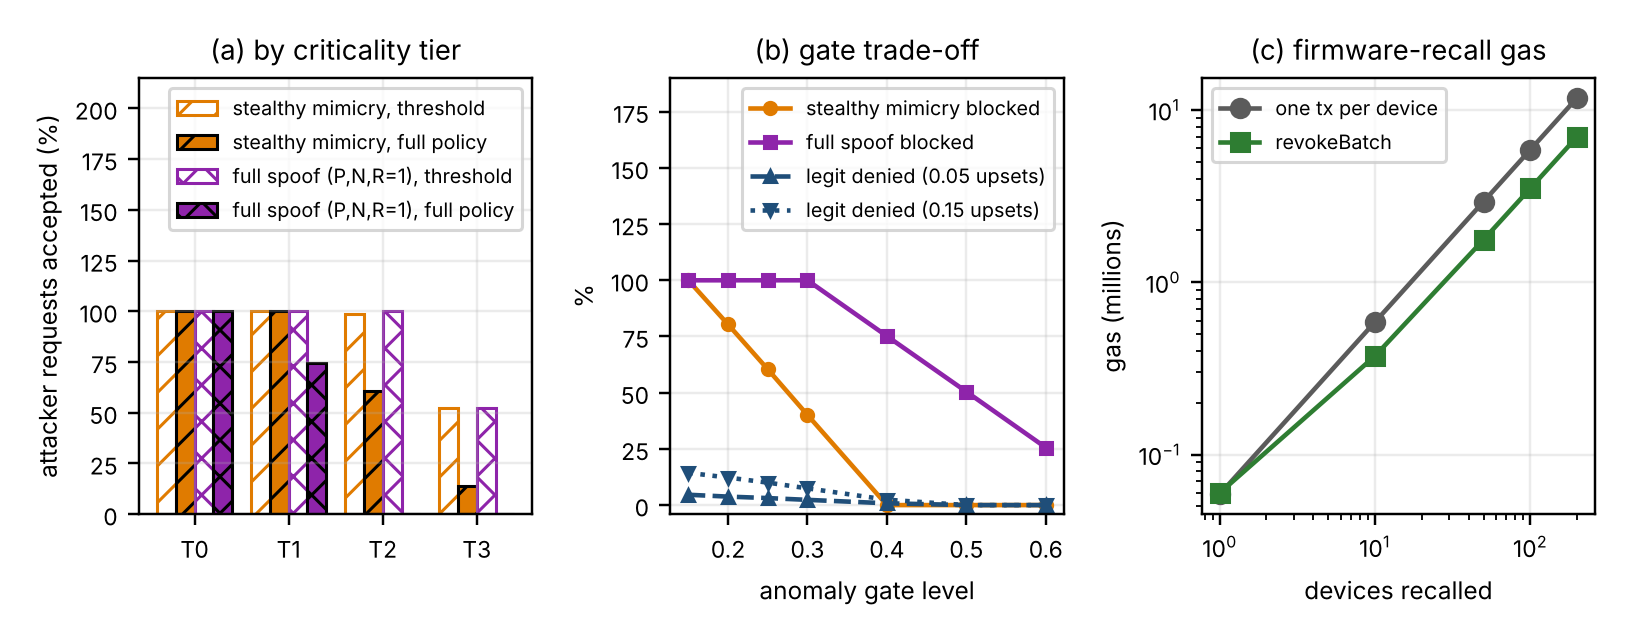
\includegraphics[width=0.72\textwidth]{../figures/fig8_iiot_results.png}
\caption{Industrial extensions: (a) attacker requests accepted per criticality tier under threshold-only and full policy; (b) anomaly-gate trade-off for 5\% and 15\% legitimate process-upset rates; (c) gas to recall devices with one transaction per device versus \texttt{revokeBatch}. Text description: in (a) the full policy accepts fewer attacker requests than the threshold-only policy for at least one attack type at each of T1--T3, and none of the full-spoof requests at T2--T3; in (b) the share of attacks blocked rises with the gate level while the share of legitimate requests denied stays below about 15\%; in (c) recall by \texttt{revokeBatch} uses less gas than one transaction per device for every fleet larger than one device. Bars and lines are distinguished by hatching and markers as well as colour.}
\label{fig:iiotres}
\end{figure*}

\paragraph{WUSTL-IIOT-2018 (SCADA).}\label{sec:wustl_eval} To check that the gate behaviour is not specific to one collection, we repeat the experiment on WUSTL-IIOT-2018 \cite{teixeira2018scada,teixeira2018wustl}. The file has 7{,}037{,}983 rows but only 62{,}959 distinct ones (99.1\% duplicates) and a binary label only, so we de-duplicate before splitting and cannot repeat the held-out-type test. The supervised classifier is almost perfect (AUC 0.99998) because attack flows here are short; an Isolation Forest on normal flows reaches $0.909\pm0.006$, a more realistic stand-in for an unseen attack. With the supervised score the full policy accepts at most 0.3\% of attack requests at T1--T3 and denies at most 0.2\% of legitimate ones. With the unsupervised score it cuts attack acceptance at T2 and T3 from 100\% and 94.1\% to 8.2\% and 4.3\%, but legitimate allowance drops to 87.5\% and 82.2\%, and an adaptive attacker sending its best 10\% (1\%) of flows is accepted 86.9\% (100\%) of the time at T2 and 43.0\% (100\%) at T3, against 2.1\% (16.0\%) and 0.7\% (6.3\%) with the supervised score. With a weak detector the policy trades a large share of legitimate availability for protection at the critical tiers.

\subsection{A Third Dataset With Attack Types: WUSTL-IIoT-2021}\label{sec:wustl21_eval}
WUSTL-IIoT-2021 contains Argus flow records from an industrial Modbus testbed with four labelled attack types \cite{zolanvari2019vulnerability,zolanvari2021wustl}, so it supports the held-out-type test the SCADA file could not. It has 1{,}194{,}464 rows (1{,}107{,}448 normal; DoS 78{,}305, reconnaissance 8{,}240, command injection 259, backdoor 212), captured on one day from two to four attacker hosts. We drop timestamps, IP addresses, the source port, \texttt{IdleTime} (an epoch timestamp that separates types by capture time) and the IP-identification fields, keep 39 features, and remove 41{,}645 exact duplicates. The protocol follows Section~\ref{sec:real_eval}.

The supervised classifier is almost perfect on seen types (AUC 0.99999); the Isolation Forest reaches $0.987\pm0.001$ because normal Modbus polling is very regular. With a type held out, the classifier flags only 0.7\% of DoS test flows at 0.5 (AUC against normal 0.71) and 8.1\% and 13.0\% of command injection and reconnaissance, although their AUC exceeds 0.999. The ranking is right, but the scores sit far below any useful gate. Backdoor is found at 66.7\%. With seen types the full policy admits 3.6--4.2\% of attack requests at T1--T3 and denies no legitimate request. With types withheld, acceptance rises to 75.4--77.8\% on average and 97.9--99.2\% for DoS, so on unseen types the supervised score adds almost nothing, and an adaptive attacker is always accepted. The unsupervised score behaves differently: the full policy admitted no attack request of any type at T1--T3, even for the best 1\% of an adaptive attacker's flows, at the price of denying 1.5\%, 12.1\% and 22.3\% of legitimate requests at T1, T2 and T3. A supervised detector does not protect against unseen attack types, and one trained on normal traffic can, but only when normal traffic is as regular as in this laboratory testbed, whose machine-generated traffic and volumetric attacks make anomaly detection easier than in a plant. The rarest attack types have very few flows (74 and 63 test flows), and posture, network context and device pairing remain synthetic.

\begin{table}[t]
\centering
\caption{WUSTL-IIoT-2021: legitimate requests allowed and attack requests accepted (\%) under the full policy, as means over four attack types; ``Thr.-only'' is the threshold-only policy on the held-out supervised scores}
\label{tab:wustl21}
\scriptsize
\setlength{\tabcolsep}{2.5pt}
\begin{tabular}{@{}lrrrrrr@{}}
\toprule
 & \multicolumn{3}{c}{Supervised $A$} & \multicolumn{2}{c}{Isolation Forest $A$} & \\
\cmidrule(lr){2-4}\cmidrule(lr){5-6}
Tier & Legit & Seen & Held-out & Legit & Attack & Thr.-only$^{a}$ \\
\midrule
T0 & 100.0 & 100.0 & 100.0 & 99.4 & 100.0 & 100.0 \\
T1 & 100.0 & 3.6 & 77.8 & 98.5 & 0.0 & 100.0 \\
T2 & 100.0 & 3.8 & 75.6 & 87.9 & 0.0 & 78.0 \\
T3 & 100.0 & 4.2 & 75.4 & 77.7 & 0.0 & 77.8 \\
\bottomrule
\end{tabular}
\end{table}

\subsection{Baselines: Revocation Exposure, Class Models and Weights}\label{sec:baselines}
On a shared logical clock we compare the per-request design with a session token (HMAC bearer token, TTL 60 or 300\,s) and PKI with a CRL refreshed every 60 or 300\,s, for 60 devices at 1 request/s with revocation times drawn from $U(100,500)$\,s. Table~\ref{tab:base} shows that the audited design accepts no request after revocation, as Proposition~\ref{prop:revoke} predicts, whereas the baselines accept on average 33 and 147 requests for the 60\,s and 300\,s windows (worst cases 59--299). Token validation is cheaper per request, which we do not hide. The fast path trades the zero for a bounded exposure of at most $\rho\Delta$ requests (Proposition~\ref{prop:stale}): with $\Delta=5$\,s and one request per second, 5 requests.

\begin{table}[t]
\centering
\caption{Revocation exposure (requests accepted after revocation; 60 devices, 1 req/s) and mean decision latency}
\label{tab:base}
\scriptsize
\begin{tabular}{@{}lrrr@{}}
\toprule
\textbf{Scheme} & \textbf{Mean exp.} & \textbf{Max exp.} & \textbf{Lat. (ms)} \\
\midrule
Session token (TTL 60 s) & 32.5 & 59 & 0.005 \\
Session token (TTL 300 s) & 146.5 & 299 & 0.006 \\
PKI$+$CRL (refresh 60 s) & 33.5 & 60 & 0.074 \\
PKI$+$CRL (refresh 300 s) & 146.5 & 299 & 0.094 \\
\textbf{Proposed (per-request)} & 0.0 & 0 & 0.070 \\
\bottomrule
\end{tabular}
\end{table}

Three further baselines answer the objection that tokens and CRLs are weak comparators (30 runs, same revocation times). Short-lived certificates and OCSP stapling bound exposure by the validity window because a revoked device cannot renew; in our model they have identical exposure (29.0 requests for 60\,s, 140.8 for 300\,s). A centralised online policy decision point that checks a revocation database on every request matches the audited path with zero exposure, so exposure alone does not favour the blockchain design against it. The differences lie elsewhere. The central PDP is a single operator that alone can revoke, reinstate or silently alter its log, and its log has no external anchor. If it is unreachable for 60\,s it must either deny every request (86.7\% of legitimate requests served) or accept requests from devices revoked meanwhile (21.0 on average, up to 60). Our fast path faces the same outage trade-off for revocations that happen while the replica is blind (Section~\ref{sec:outage_eval}), so the claim we can support concerns governance and auditability, not availability. The simulation models validity windows only.

\paragraph{Architecture-class baselines.}\label{sec:prior_eval} To compare against the \emph{design choices} of earlier blockchain schemes we added two class models, built from how each family is described in the literature and run in the same simulator; they are not re-implementations of any named system. The first is a ledger registry checked at login, after which a session is trusted (the authenticate-once pattern \cite{wang2026medicaliot,james2024authz}): with 60\,s and 300\,s sessions a revoked device is still accepted for a mean of 29.0 and 129.2 requests (maxima 60 and 300). Putting the registry on a ledger therefore does not close the window unless every request is checked. The second is an on-chain policy with one static threshold of 0.55 for every resource. Table~\ref{tab:prior} shows that at the two critical tiers it accepts every partial-mimicry, stealthy and fully spoofed request, since a fully spoofing attacker scores at least 0.70 (Section~\ref{sec:security}), whereas the full policy accepts 0\%, 60.9\% (T2) and 13.6\% (T3) of the three attacks at a cost of 2.2\% and 5.2\% of legitimate requests.

\begin{table}[t]
\centering
\caption{Static single-threshold on-chain policy (class model) versus the full policy at the two critical tiers (synthetic fleet, 4{,}000 requests per population)}
\label{tab:prior}
\scriptsize
\setlength{\tabcolsep}{2.5pt}
\begin{tabular}{@{}llrrrr@{}}
\toprule
& & Legit. & \multicolumn{3}{c}{Attack accepted (\%)} \\
\cmidrule(lr){4-6}
\textbf{Policy} & \textbf{Tier} & denied (\%) & Partial & Stealthy & Full spoof \\
\midrule
Static threshold 0.55 & T2 & 0.0 & 100.0 & 100.0 & 100.0 \\
Full policy (this paper) & T2 & 2.2 & 0.0 & 60.9 & 0.0 \\
Static threshold 0.55 & T3 & 0.0 & 100.0 & 100.0 & 100.0 \\
Full policy (this paper) & T3 & 5.2 & 0.0 & 13.6 & 0.0 \\
\bottomrule
\end{tabular}

\end{table}

\paragraph{Weight sensitivity.} The synthetic weights $(0.30,0.30,0.20,0.20)$ were chosen by hand, so we moved each by $\pm0.10$ (rescaling the others) and drew 200 random perturbations. At T2 legitimate denial stayed between 2.2\% and 2.3\% and stealthy acceptance between 60.5\% and 60.9\%. At T3 legitimate denial ranged from 3.4\% to 11.8\% (median 5.7\%) and stealthy acceptance from 11.8\% to 14.8\%. Partial-mimicry and full-spoof acceptance stayed at 0\% in every variant. The gate therefore holds for any reasonable weighting, while the false-denial cost at the highest tier depends on the weights and should be tuned per plant.

\subsection{Firmware Recall Capacity}\label{sec:recall_eval}
Table~\ref{tab:recall} reports gas for revoking $k$ devices with one transaction each and with \texttt{revokeBatch}; \texttt{suspendBatch} is shown for quarantine. For one device the batch call is 1.7\% dearer, but from ten devices on it saves 36.5--40.5\%, approaching about 35k gas per device against 58.9k. In 30M-gas blocks, recalling $10^4$ devices needs about 20 blocks with individual transactions and 12 with batches, and $5\times10^4$ devices need 99 and 59 (other traffic is not modelled). Devices revoked in later blocks stay exposed until their block, so the highest-criticality devices should go first. A recall approved by quorum adds the vote overhead and executes through \texttt{executeBatch}: 100 devices cost 3.81M gas and 200 devices 7.30M gas in total, about 36.5k gas per device (a fleet of $10^4$ is still about 12 blocks), and a quorum reinstatement with $N=5$ costs 291k gas.

\begin{table}[t]
\centering
\caption{Gas for recalling devices: one transaction per device versus \texttt{revokeBatch}, and \texttt{suspendBatch}}
\label{tab:recall}
\scriptsize
\begin{tabular}{@{}rrrrr@{}}
\toprule
Devices & One tx each & \texttt{revokeBatch} & Saving & \texttt{suspendBatch} \\
\midrule
1 & 58{,}836 & 59{,}859 & -1.7\% & 31{,}626 \\
10 & 588{,}336 & 373{,}725 & 36.5\% & 98{,}907 \\
50 & 2{,}941{,}716 & 1{,}768{,}637 & 39.9\% & 397{,}903 \\
100 & 5{,}883{,}408 & 3{,}512{,}289 & 40.3\% & 771{,}717 \\
200 & 11{,}766{,}864 & 6{,}999{,}533 & 40.5\% & 1{,}519{,}165 \\
\bottomrule
\end{tabular}
\end{table}

\subsection{Attack Detection}\label{sec:attacks}
Replay, forged-signature, use-after-revocation and unregistered-DID probes were each run in 500 trials and denied every time (one-sided 95\% upper bound on failure 0.6\%). This validates the state-machine logic against these attacks; it is not evidence of unconditional security.

\subsection{Decentralized Revocation Governance}\label{sec:governance_eval}
Table~\ref{tab:governance} evaluates \texttt{RevocationGovernance} for $N\in\{5,7,9,11,15,21\}$ with 200 trials per size. Mean quorum latency grows roughly linearly, from 0.56\,ms ($N=5$) to 1.91\,ms ($N=21$) for a cooperative group and from 0.93 to 3.67\,ms under maximal tolerated dissent ($N-q$ DENY voters). In all 1{,}200 trials the dissenting minority never prevented approval, and in 1{,}200 forced-revocation attempts with only $q-1$ approvals no revocation executed, consistent with Proposition~\ref{prop:gov}. On the EVM a proposal costs 76k gas, each vote 78k and the final vote 103k, so a quorum revocation costs 317k ($N=5$) to 805k gas ($N=21$): governance cost grows with $q$, not with the fleet. Kumar et al.\ report 3--4\,s for registration and under 5\,s for revocation on a live PoA chain \cite{kumar2026privacy}; our figures measure compute only and are not comparable like for like. In a deployment each vote is a transaction, so revocation takes about $q$ block confirmations when votes are sequential, or one to two blocks when they are parallel.

\begin{table}[t]
\centering
\caption{Governance: mean testbed latency (ms) cooperative and under maximal dissent; \% trials where maximal dissent still reached quorum (Appr.); \% where a $q-1$ coalition executed a revocation (Forced); EVM gas for one quorum revocation}
\label{tab:governance}
\scriptsize
\begin{tabular}{@{}rrrrrrr@{}}
\toprule
$N$ & $q$ & Coop. & Dissent & Appr.\% & Forced\% & Total gas \\
\midrule
5 & 3 & 0.562 & 0.926 & 100 & 0 & 317{,}162 \\
7 & 4 & 0.667 & 1.166 & 100 & 0 & 378{,}152 \\
9 & 5 & 0.803 & 1.440 & 100 & 0 & 439{,}142 \\
11 & 6 & 0.946 & 1.729 & 100 & 0 & 500{,}120 \\
15 & 8 & 1.299 & 2.438 & 100 & 0 & 622{,}112 \\
21 & 11 & 1.909 & 3.665 & 100 & 0 & 804{,}950 \\
\bottomrule
\end{tabular}
\end{table}

\subsection{End-to-End Evaluation on a Four-Validator QBFT Network}\label{sec:besu_eval}
To move beyond in-process execution we deployed the three contracts on a private Hyperledger Besu 25.7.0 network of four QBFT validators (2\,s block period, 4\,s round-change timeout). We drove it through JSON-RPC with signed transactions. We ran it first with all validators and the load generator on one two-vCPU container, then \label{sec:gcp_eval}on Google Cloud with one validator per e2-standard-2 virtual machine in europe-west3, us-east4, asia-southeast1 and southamerica-east1. We injected no artificial delay and did not record round-trip times, so the delay is whatever the provider's network gave on the day of the run (2026-10-12). Table~\ref{tab:gcp} sets the two runs side by side; both are single runs of the same script.

\emph{Finality and replica lag.} Every state-changing call needs about one block period from submission to receipt (1.98--2.00\,s on average, p95 about 2.2\,s) in both deployments; QBFT finalizes in the block that includes the transaction. Inter-region distance did not push consensus beyond one block period. A revocation became visible on a second validator after 1.87\,s on one host and 1.76\,s across regions, and 30 of 30 audited decisions issued afterwards returned DENY. On one host the replica was up to date before the receipt poll returned ($-117\pm75$\,ms); across regions it trailed the receipt by $+212\pm145$\,ms (p95 362\,ms, maximum 495\,ms). For this network, the exposure bound $\rho\Delta$ of Proposition~\ref{prop:stale} is therefore dominated by the block period plus 0.2--0.5\,s; a plant link over a public network or satellite path would give a larger $\Delta$ and has to be measured where it is deployed.

\emph{Throughput.} Pre-signed audited decisions from ten accounts were all mined at 100, 300 and 600 offered. Sustained throughput was 11--18 tx/s on one host (mean latency 31.6\,s at 600 offered) and 30.8, 34.4 and 50.1 tx/s across regions (8.6\,s). The regional figure is a lower bound, since throughput still rose with load, and both are well below the gas-based ceiling of 213 decisions per second; we did not determine what limits them. We recorded no network round-trip times and did not determine what limits throughput, so the figures describe this setup, not the design's capacity. The conclusion for the design is unchanged: routine requests must not wait for consensus.

\begin{table}[t]
\centering
\caption{The same benchmark on one host and with one validator in each of four Google Cloud regions (mean $\pm$ sd; single runs)}
\label{tab:gcp}
\scriptsize
\setlength{\tabcolsep}{3pt}
\begin{tabular}{@{}lrr@{}}
\toprule
Measurement & One host & Four regions \\
\midrule
Block interval (s) & 2 $\pm$ 0 & 2 $\pm$ 0 \\
\texttt{register}, submit$\to$receipt (ms) & 1977 $\pm$ 139 & 1980 $\pm$ 162 \\
\texttt{evaluateAccess}, submit$\to$receipt (ms) & 1997 $\pm$ 125 & 1997 $\pm$ 134 \\
\texttt{anchorDecisions}, submit$\to$receipt (ms) & 1993 $\pm$ 127 & 1993 $\pm$ 130 \\
Revocation, submit$\to$receipt (ms) & 1985 $\pm$ 121 & 1552 $\pm$ 169 \\
Revocation, submit$\to$visible on replica (ms) & 1868 $\pm$ 85 & 1764 $\pm$ 211 \\
Replica minus receipt (ms) & -117 $\pm$ 75 & 212 $\pm$ 145 \\
Quorum revocation $N{=}5,q{=}3$, sequential (s) & 8.07 $\pm$ 0.24 & 8.17 $\pm$ 0.14 \\
Quorum revocation $N{=}5,q{=}3$, parallel (s) & 4.03 $\pm$ 0.12 & 4.33 $\pm$ 0.13 \\
\texttt{revokeBatch}, 50 devices, receipt (s) & 2.95 & 2.41 \\
\texttt{revokeBatch}, 200 devices, receipt (s) & 6.13 & 2.99 \\
Throughput, 100 offered (tx/s) & 17.8 & 30.8 \\
Throughput, 300 offered (tx/s) & 16.0 & 34.4 \\
Throughput, 600 offered (tx/s) & 11.3 & 50.1 \\
Mean latency at 600 offered (s) & 31.6 & 8.6 \\
\bottomrule
\end{tabular}
\end{table}

\emph{Governance and recall.} A three-of-five revocation took 8.07\,s (one host) and 8.17\,s (regions) with sequential votes, and 4.03\,s and 4.33\,s with parallel votes, about four and two blocks. Revoking 50 and 200 devices in one transaction (1.77M and 7.00M gas) was confirmed after 2.95 and 6.13\,s on one host and 2.41 and 2.99\,s across regions, whereas registering 200 devices one by one took 399\,s. The number of blocks, not the number of transactions, determines recall and governance latency.

\emph{Fault tolerance.} With four validators QBFT tolerates one fault. With one validator stopped, registration averaged 2.83\,s on one host and $3.43\pm2.17$\,s across regions against 1.97\,s at baseline, because rounds in which the stopped validator was the proposer had to time out. With two stopped no block was produced, and a pending transaction was mined 78\,s (one host) and 75\,s (regions) after restart. These runs used one pending transaction and few samples; we did not test partitions, injected delay or validators in one region. During a halt the fast path keeps deciding on its last replicated state, and the outage policy of Section~\ref{sec:outage} governs what is allowed.

\subsection{Ablation, Exposure from the Decision Time, and Calibrated Gates}\label{sec:review_eval}
These three experiments (\texttt{sim/experiments\_review.py}) answer questions that the earlier results left open; all use the same populations, seeds and tiers as above unless stated.

\paragraph{Which component does the work?}\label{sec:ablation2} We compare the full policy with its parts on the synthetic fleet (4{,}000 requests per population, a separate draw from Section~\ref{sec:gate_eval}, so the figures differ slightly). Each alternative is tuned so that it admits the same share of legitimate requests as the full policy, which makes the attack columns comparable. Table~\ref{tab:ablate2} gives the result. The gate carries the effect: at T2 and T3 the threshold alone admits 100\% and 53\% of full spoofing, and adding the gate reduces both to 0\%. Strict mode adds nothing once the gate is present; on its own it only removes the STEP\_UP outcome (at T3 the threshold alone returns ALLOW or STEP\_UP for 85.5\% of full spoofing, against 53.0\% ALLOW). Raising the threshold until legitimate cost matches the gate does not help against full spoofing (58.1\% and 49.0\% still accepted), as Proposition~\ref{prop:bound} predicts. A non-linear score, the minimum of $P$, $1-A$, $N$ and $R$, reaches the same effect without a separate gate (0\% of full spoofing at T2 and T3) and is better than the gate at T1 (38.0\% against 75.3\%). So the evidence supports the principle that the anomaly signal must be able to veto independently of a linear sum; it does not show that a hard gate is the only or best way to do so. Stealthy mimicry, which keeps $A$ low, is not stopped by any variant (18.8--61.1\% still accepted at T2--T3).

\begin{table}[t]
\centering
\caption{Ablation at matched legitimate allowance: attack requests accepted (\%), ALLOW only (4{,}000 requests per population, one seed). Full = gate and strict mode}
\label{tab:ablate2}
\scriptsize
\setlength{\tabcolsep}{3pt}
\begin{tabular}{@{}lrrrrrrrr@{}}
\toprule
& \multicolumn{4}{c}{T2 plc.setpoint.write} & \multicolumn{4}{c}{T3 plc.firmware.update} \\
\textbf{Policy} & Legit. & Partial & Stealthy & Spoof & Legit. & Partial & Stealthy & Spoof \\
\midrule
Threshold only & 99.8 & 53.6 & 98.0 & 100.0 & 95.2 & 7.7 & 53.2 & 53.0 \\
Strict only & 99.8 & 53.6 & 98.0 & 100.0 & 95.2 & 7.7 & 53.2 & 53.0 \\
Gate only & 97.2 & 0.0 & 61.1 & 0.0 & 93.6 & 0.0 & 18.8 & 0.0 \\
Full (gate + strict) & 97.2 & 0.0 & 61.1 & 0.0 & 93.6 & 0.0 & 18.8 & 0.0 \\
Raised threshold & 97.2 & 9.9 & 57.5 & 58.1 & 93.6 & 6.2 & 47.9 & 49.0 \\
Min-of-signals score & 97.2 & 0.0 & 60.7 & 0.0 & 93.6 & 0.0 & 54.6 & 0.0 \\
\bottomrule
\end{tabular}
\end{table}

\paragraph{Exposure counted from the decision time.}\label{sec:exposure_eval} The baselines in Table~\ref{tab:base} count exposure from the moment the revocation is decided, whereas the on-chain figure of zero counts from finalization, which is not a like-for-like comparison. We therefore redraw the revocation delay from the measured Besu distributions (submission to receipt for the audited path, submission to visibility on another validator for the fast path; 30 samples each) and count the requests a device sends at 1 per second after the revocation transaction was \emph{submitted}. Across four regions the audited path accepts 1.5 requests on average (at most 2) and the fast path 1.8 (at most 3); on one host the figures are 2.0 and 1.9 (at most 3 each). The audited and fast paths are therefore indistinguishable in practice, and both are far below the 33 and 147 of the token and CRL baselines (which include no block period at all), though the sample is 30 delays from one run per deployment.

\paragraph{Gates calibrated on legitimate traffic, and a host-grouped split.} The hand-set gates of Table~\ref{tab:tiers} were tuned on synthetic ranges. On TON\_IoT we now split the network flows by source host (35 hosts for training and 16 for testing, five splits), so that no host appears on both sides, and we set one gate at the 99th percentile of half of the legitimate scores, evaluating on the other half. The supervised detector remains strong (AUC 0.999) and the calibrated gate admits 0.4--0.5\% of attack requests with 99.7\% or more of legitimate requests allowed at T1--T3. The Isolation Forest is weaker under this split (AUC 0.874). Its calibrated gate (0.69) lets 91.8, 91.5 and 65.0\% of attack requests through at T1--T3, against 76.9, 40.5 and 34.7\% for the hand-set gates, which cost 2.0, 14.1 and 19.5\% of legitimate requests. On WUSTL-IIoT-2018 with an Isolation Forest trained on normal flows, the hand-set gates admit 100, 9.4 and 4.2\% of attacks while denying 3.6, 13.8 and 18.5\% of legitimate requests. The calibrated gate (0.97) admits 100, 100 and 94.5\% with 1.7, 7.0 and 15.2\% denied. On the original stratified TON\_IoT split with the supervised detector, the calibrated gate (0.27) admits 0.3\% of seen-type attacks and 7.4\% of held-out types on average, but up to 34.6\% for the worst type. A gate set from legitimate data alone therefore cannot be assumed to protect: where attack scores overlap the legitimate tail, the false-denial budget decides how much attack traffic passes, and the gate must be tuned with attack-like data or accepted as weak.

\subsection{Static Analysis and Randomised Invariant Tests}\label{sec:assure}
Slither (102 detectors) reported 11 findings on the three contracts: one medium (a strict equality on \texttt{registeredAt==0}, the intended existence test), four low, one informational finding per signature-recovery routine and four optimisation hints. No reentrancy, access-control or arithmetic finding was reported. Reading the code, we found one genuine gap: with a zero oracle address or a zero registered signer, an invalid signature (for which \texttt{ecrecover} returns the zero address) would pass. We added a zero-oracle check in the constructor and rejected a zero recovered address at registration (+62 gas for \texttt{registerDevice}). Three new tests complement the 13 unit tests, including a randomised state-machine test (300 steps, three seeds, six devices) against an independent model; four further tests cover governor-only revocation, suspend-only single-party action, quorum recall and expired attestations; all 20 pass. The Slither run predates the hardening described in Section~\ref{sec:governance} and has not been repeated. This is bounded random testing, not a proof or audit; the contracts are not formally verified.

\subsection{Degraded Operation During an Outage}\label{sec:outage_eval}
We applied the policy of Section~\ref{sec:outage} to 400 devices at one request per second, a quarter of them T2 clients, with 10\% of devices revoked at random times during an outage starting at $t=200$\,s of 600\,s. A fully fail-closed PEP stops serving everyone, so availability falls to 89.9\% for a 60\,s outage and 50.4\% for 300\,s. The degraded policy keeps T0--T1 running (99.4\% and 97.0\%) but denies every T2 request and accepts requests from devices revoked while it was blind (962 for 60\,s, 4{,}398 for 300\,s). The scenario is deterministic given its parameters, so it illustrates the trade-off rather than measuring it: the operator chooses explicitly between unsafe acceptances and lost availability.
